\documentclass[conference]{IEEEtran}
\IEEEoverridecommandlockouts

\usepackage{cite}
\usepackage{amsmath,amssymb,amsfonts}
\usepackage{algorithmic}
\usepackage{graphicx}
\usepackage{textcomp}
\usepackage{xcolor}
\usepackage{hyperref}

\begin{document}

\title{Know your enemy and know yourself}
% \subtitle{Detecting AI generated text with source model prediction}
\author{
  \IEEEauthorblockN{Bo-Yi Mao}
  \IEEEauthorblockA{
    \textit{Dept. of Computer Science} \\
    \textit{National Tsing-Hua University}\\
    Hsinchu, Taiwan
  }
  \and
  \IEEEauthorblockN{Aurick}
  \IEEEauthorblockA{
    \textit{Dept. of Computer Science} \\
    \textit{National Tsing-Hua University}\\
    Hsinchu, Taiwan
  }
  \and
  \IEEEauthorblockN{Kenneth}
  \IEEEauthorblockA{
    \textit{Dept. of Computer Science} \\
    \textit{National Tsing-Hua University}\\
    Hsinchu, Taiwan
  }
  \and
  \IEEEauthorblockN{Yi-Hsueh Chu}
  \IEEEauthorblockA{
    \textit{Dept. of Computer Science} \\
    \textit{National Tsing-Hua University}\\
    Hsinchu, Taiwan
  }
}

\maketitle

\section{Introduction}

With the recent boom of generative models and large language models (LLMs), their potential has enabled plagiarism in academic writing. The Detect AI Generated Text (DAIGT) competition hosted on Kaggle \cite{daigt} aims to identify and discriminate AI-generated essays to ensure fairness in the usage of LLMs.

Previous works mostly focus on improving training data quality and diversity and using larger and larger models. However, few have attempted to address the distribution difference of different language models. In this paper, we present our approach to detecting AI-generated text by predicting the source model used to generate the text. We explore various machine learning techniques and natural language processing (NLP) methods to achieve this goal. Our contributions include a comprehensive dataset of AI-generated and human-written texts, a detailed analysis of different models' performance, and insights into the features that distinguish AI-generated text from human-written text.

\section{Previous Works}

Transformer-based classification models often struggle to generalize from the PERSUADE corpus dataset to the secret test dataset, frequently tending towards overfitting. As a result, many attempts have resulted in scores around 0.75, despite performing well on local validation. Consequently, many have found other approaches to tackling the problem.

One notable success from Bamba et al. \cite{1stplace} involved increasing both the diversity and size of the training dataset. Yhey achieved a significant improvement in accuracy by leveraging a diverse and extensive dataset. They utilized a combination of AI-generated and human-written texts, which helped in training robust models capable of distinguishing between the two, eventually winning the competition at first place, with a score of 0.988.

Another work from James Day \cite{5thplace} used 500,000 documents from The Pile and another 500,000 plausible continuations generated with local LLMs, and resulted in a sizeable increase in accuracy; in fact, they submitted a DeBERTa-v3 LLM at a context length of 1024 tokens with scores of 0.96 for individual models and 0.963 for an ensemble. Compared to the models trained on the PERSUADE corpus, which scored around 0.75, this is a significant improvement.

However, Davide Cozzolino \cite{6thplace} took a different approach by using synthetic feature such as entropy, surprisal, and average word length. By merely focusing on these features, Cozzolino was able to achieve a competitive score in the DAIGT competition. As shown in Figure \ref{fig:cozzolino}, his method demonstrated that even without relying heavily on large datasets or complex models, it is possible to achieve good performance by carefully selecting and engineering features that capture the nuances of AI-generated text.

\begin{figure}[htbp]
  \centerline{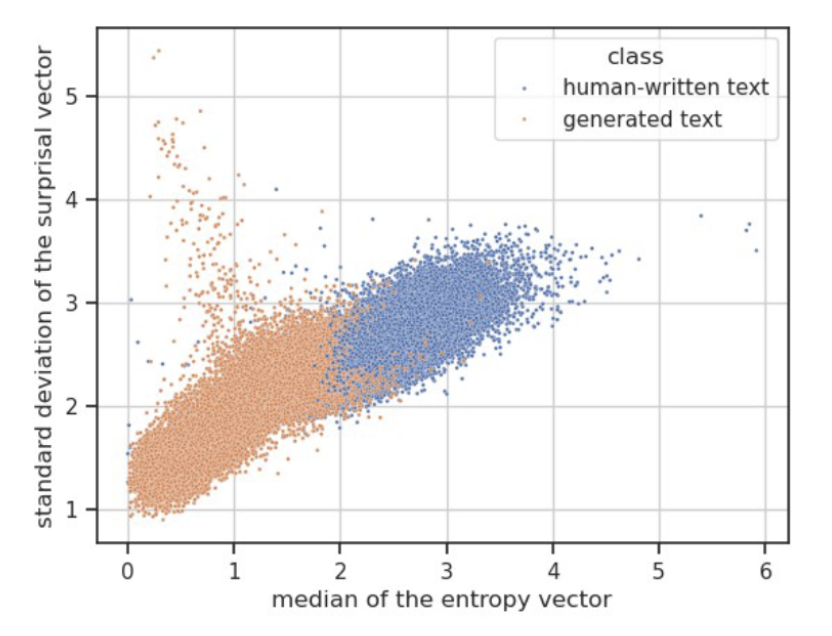
\includegraphics[width=\columnwidth]{figs/cozzolino.png}}
  \caption{Engineered features used by Davide Cozzolino \cite{6thplace} separates AI-generated text from human-written text well.}
  \label{fig:cozzolino}
\end{figure}

\section{Methodology}

Our methodology overall consists of three steps. First, the data is prepared and preprocessed ahead of time, published to Kaggle, and ready to be used. Second, certain representation learning models perform feature extraction on raw data. Finally, binary/multi-class classification is performed via various machine learning methods.

\subsection{Data Preparation}

We collected training data from several sources \cite{persuade,mistral7b,argugpt,daigtv4,fpeprocessed}, containing 87k AI-generated and 13k human-written essays, with prompts from PERSUADE, WECCL, TOEFL, and GRE corpus. The generated essays are generated from various models, including T5, LLaMA series, GPT series, Mistral7B, Claude, Falcon, T5, PaLM, and Cohere. The class distributions (AI-generated vs. human-written) are shown in Figure \ref{fig:class_dist}, and the distribution of source models is shown in Figure \ref{fig:source_dist}.

\begin{figure}[htbp]
  \centerline{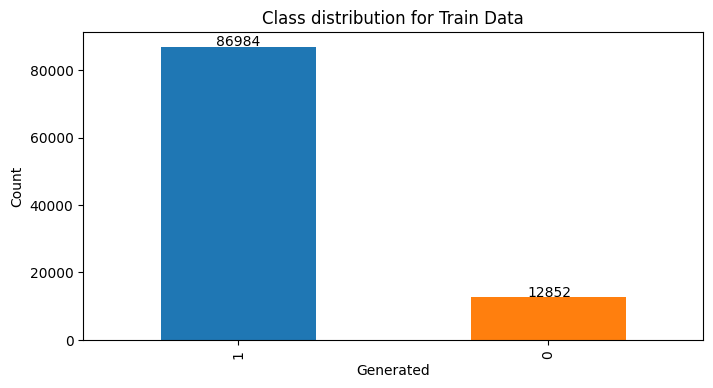
\includegraphics[width=\columnwidth]{figs/class_dist.png}}
  \caption{Class distribution of AI-generated and human-written essays}
  \label{fig:class_dist}
\end{figure}

\begin{figure}[htbp]
  \centerline{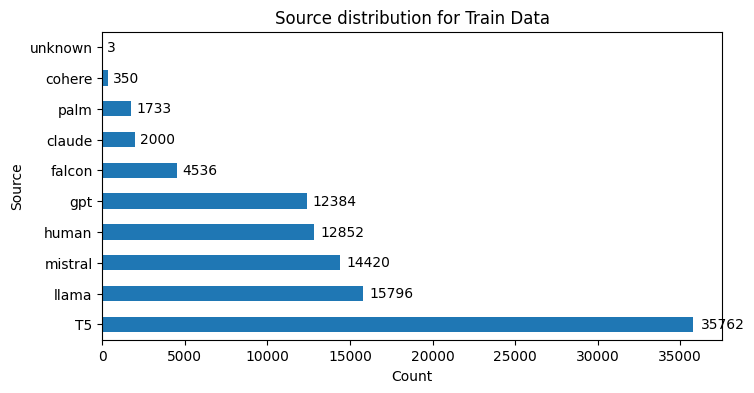
\includegraphics[width=\columnwidth]{figs/source_dist.png}}
  \caption{Distribution of source models}
  \label{fig:source_dist}
\end{figure}

\subsection{Text Tokenization}

\subsection{Feature Extraction}

% TF-IDF document vectorization is proven to be useful in various text classification tasks…

Term Frequency-Inverse Document Frequency (TF-IDF) is a popular technique for document vectorization, which is proven to be useful in various text classification tasks. We use TF-IDF to extract features from the text data, which are then used as input to the classifier. The TF-IDF vectorizer is trained on the training data and used to transform both the training and test data.

% (Aurick, 6th place sol, entropy and surprisal-based features)
% (Ethan, LLM embedding model)


\subsection{Classification}

\section{Experiments}

As the competition is a code competition, we have to submit our code to Kaggle for evaluation. We have tested various models and hyperparameters, as shown in Table \ref{tab:models}. The best model we have found is\dots

\begin{table*}[htbp]
  \centering
  \caption{Tested models and their respective accuracies}
  \label{tab:models}
  \begin{tabular}{p{1.8cm}p{1.5cm}p{2.3cm}p{3cm}p{3cm}p{1.6cm}p{1.6cm}}
    \hline
    \textbf{Training Set} & \textbf{Tokenizer} & \textbf{Feature Extractor} & \textbf{Classifier} & \textbf{Hyperparameters} & \textbf{Private Score} & \textbf{Public Score} \\
    \hline
    Ours & BPE & TF-IDF & Multi-class ensemble & human\_factor=$3 \times 10^4$ & 0.807771 & 0.912862 \\
    Ours & BPE & TF-IDF & Multi-class ensemble & human\_factor=$1 \times 10^5$ & 0.782545 & 0.898491 \\
    Ours & BPE & TF-IDF & Multi-class ensemble & human\_factor=$0$ & 0.770701 & 0.920051 \\
    Ours & BPE & TF-IDF & Multi-class ensemble & human\_factor=$1 \times 10^{-3}$ & 0.760378 & 0.919360 \\
    Ours & BPE & TF-IDF & Binary ensemble & lower=False & 0.665908 & 0.891152 \\
    Ours & BPE & TF-IDF & Binary ensemble & lower=True & 0.658713 & 0.894109 \\

    Ours & Mistral & Mistral7b & Mistral7b & - & 0.702772 & 0.854477 \\
    Base & Mistral & Mistral7b & Mistral7b & - & 0.53 & 0.54 \\
    \hline
    % (decision tree + linear classifier + multinomial naive bayes)
  \end{tabular}

  \vspace{0.5cm}

  \begin{tabular}{ll}
    \hline
    \textbf{Classifier} & \textbf{Description} \\
    \hline
    Multi-class ensemble & ensemble of linear classifier, multinomial naive bayes, and LightGBM, classifying source model \\
    Binary ensemble & ensemble of linear classifier, multinomial naive bayes, and LightGBM, with binary classification \\
    Base & Baseline model \\
    \hline
    
  \end{tabular}
\end{table*}

% discussion

\section{Conclusion}

\section{Data and Code Availability}

Our own dataset is available on Kaggle at \url{https://www.kaggle.com/datasets/dogeon188/daigt-datamix}. The code for our experiments is available on GitHub at \url{https://github.com/Dogeon188/NLP-term-daigt}.

\bibliographystyle{IEEEtran}
\bibliography{refs}

\end{document}